\chapter {Planning}

\section {Chemical Ideas}


	\subsection{Rate of Reactions}

The definition of the rate of reaction is the rate at which reactants are converted into products. This has the mathematical equation of $Rate = \frac{\Delta Concentration}{Time}$. Finding the rate of reaction obtained by studying the chemical kinetics of a specific reaction. The rate of reaction gives you important information such as whether a reaction takes place at all or how fast a reaction will occur. These chemical ideas are very important in the chemical industry as they allow for companies to reduce the cost and time in producing a product. The balanced chemical reaction only describes the stoichiometry between the reactants present and the amount of products that can be formed from them. 

	\subsection{Factors that affect Rate of Reaction}

Increasing the concentration of the reactants increases the rate of reaction, up to a terminal concentration. This can be explained as two substances physcially are unable to react with each other unless their particles come into contact with each other with enough kinetic energy (above the activation energy level). This means that if there is no contact between the particles, or the particles do not have enough kinetic energy, the rate of reaction will be zero. In contrast to this the higher the concentration of the reactants the more likely the particles are to collide above the activation energy per unit time allowing for a reaction to occur.

High temperatures allow for the particles within a system to have a greater kinetic energy. As the kinetic energy of the particles within a system increases, the particles move faster in the enclosed space, thus causing an increased chance of collision per unit time and also allowing for an increased chance of a collision above the activation energy. Virtually all reactions increase in rate if you increase the temperature. Decreasing the temperature has the opposite affect upon the rate of reaction (decreases the rate). In some systems, multiple reactions can take place, with each reaction happening at different temperatures. An example of this is the conversion of ethanol to diethyl ether, this occurs at around 100$^{\circ}$C, this is shown below:

$\mathrm{2CH_3CH_2OH}\xrightarrow{\mathrm{H_2SO_4}}\mathrm{CH_3CH_2OCH_2CH_3}+\mathrm{H_2O}$

However at 100$^{\circ}$C a different product is produced, ethylene$^1$.

$\mathrm{CH_3CH_2OH}\xrightarrow{\mathrm{H_2SO_4}}\mathrm{C_2H_4}+\mathrm{H_2O}$

Pressure only affects the rate of reaction if the reaction involves gases. Changing the pressure when a reaction involves only solids or liquids will have no effect on the rate of the reaction. Increasing the pressure of a gas is the same as increasing the gases concentration. If a given volume of gas is squeezed into a smaller volume the concentration is higher as shown by the equation:

 $p= \frac{n}{V}\times{RT}$

Where:
\begin{itemize}
\item p is pressue.
\item V is volume.
\item n is the number of moles.
\item R is the gas constant.
\item T is the temperature is K
\end{itemize}

Therefore this euqation shows that as long as the remperature is constant, the pressure is directly proportional to the concentration. If you double one, you will also double the other$^2$.

Radiation is a form of energy and therefore it may speed up the rate of reaction as it provides the particles of the reactants with more energy, therefore allowing for more collisions above the activation energy per unit time. As the intensity of radiation increases, the particles absorb more energy and in turn the rate of reaction increases.

Surface area is important in chemical kinetics as increasing the surface area of a reactant will generally increase the rate of reaction. An example of this is iron, in solid form iron is stable enough to use as solid blocks in building structures; however, in powder form a pyrotechnic composition can be created to form thermie which when ignited by heat undergoes a vigorous exothermic reduction-oxidation reaction$^3$. The reason the rate of reaction increases as the surface area of reactants increases is because there is more area exposed that can be hit by other reactant molecules, thus increasing the collisions per unit time.

When two reactants are in the same fluid pase, their particles collide more frequently than one or both reactants are solids, or when two fluids dont mix. This means that if reactants are in two different phases, collisions between the reactants only occur at the interfaces between the phases. This means that the surface area available for particles to collide is extremely small in comparison to a single homogeneous soluton amd as discussed above, a smaller surface area equates to a slower reaction time due to the reduced collisions per unit time.

Having a catalyst present in the reaction increases the rate of reaction in both the forward and reverse reactions by providing an alternative pathway of lower activation energy. This means that particles do not need as much kinetic energy to successfully collide together to create a reaction, thus allowing for more successful collisions per unit time. The catalyst, itself remains chemically unchanged. In industry most chemicals are produced using catalysts as they reduce the costs of production. For example, an iron catalyst is used for the Haber process (the process of making ammonia from nitrogen gas and hydrogen gas). This catalyst allows for a higher yield of ammonia without having to increase the temperature or pressure, which would cost a lot of money$^4$.

Ion inhibitors such as zinc activated channel antagonists or catalyst poisons decrease the rate of reaction when introduced into a reaction mixture. This is achieved by the ion inhibitors combining with the reactant molecule thus reducing the number of colliding reactants per unit time, as the surface area of the reactant is covered up. This decrease of successful collisions and hence decreases the rate of reaction. A catalyst poison also reduces the effectiveness of a catalyst. When a reaction occurs with a solid catalyst, a catalyst poison decreases the rate of reaction by accumulating on the surface of the solid catalyst. A common example of a catalyst poison is oxygen and water on an iron catalyst, commonly used in ammonia synthesis, as discussed above. Therefore as there is less surface area on the catalyst, there are less successful collisions per unit time, thus decreasing the rate of reaction.

As a general rule of thumb, introducing low amounts of colvents will increase the concentration, therefore increasing the rate of reaction. Most organic reactions are done in solution for this reason. However http://www.researchgate.net/post/How_the_solvent_effect_the_reaction_rate

	\subsection{Rate Equations}





	\subsection{Finding Rates}


Rates have to be determined experimentally. The average rate of reaction is obtained by taking the change in concentration over a specific time period. This value is only an approximation of the rate of reaction in that specific time period. This means that this method does not give you the specific rate values throughout that time interval and in some cases, that rate value is not even equal at any time throughout that time interval.

Another method called the instantaneous rate of reaction, in contrast to the average rate of reaction allows for a more accurate value to be obtained. This method is defined as the change in concentration of an infinitely small time interval. The derivative mathematical equation for this is $\frac{d[Concentration]}{dTime}$. By graphing the concentration of the experiment over time you are then able to draw a tangent line at a specific time value. The gradient of the tangent then corrospondes to the rate of reaction. You can also mix these two methods to get an average rate which is closer to the value of the instantaneous rate. This is done by measuring the change in concentration over a very small time period, two or more times to obtain an average. Again the rate of reaction for that time period is detemined by the slope of the tangent lines$^5$.





		\subsubsection{Justification of Chosen Method}

For my experiment I will be finding the rate of reaction using the following steps:

\begin{enumerate}
\item Plot a graph of the volume of hydrogen against time.
\item From the graph draw a tangent to the line at the initial point.
\item Calculate the gradient of the tangent by using the equation: 
\item The gradient is equal to the rate of reaction.
\end{enumerate}

I have chosen this method as it is the method which will give me the most accurate values for the specific point in time which I wish to measure. 


	\subsection{Orders of Reactions}





	\subsection{pH}

The pH scale is composed of two extremes that describes a chemical property about the substance being tested, these extremes are called acids and bases. Mixing acids and bases together will induce a neutralisation reaction which can cancel out their extreme effects. A substance which is neither acidic nor basic is called a neutral substance. The pH scale ranges from 0 to 14, with 0 being as acidic as possible and 14 being as basic as possible. Neutral has a corresponding pH of 7 and therefore anything below 7 is acidic and anything above 7 is basic. The pH scale is illistrated below.


\begin{figure}[H]
    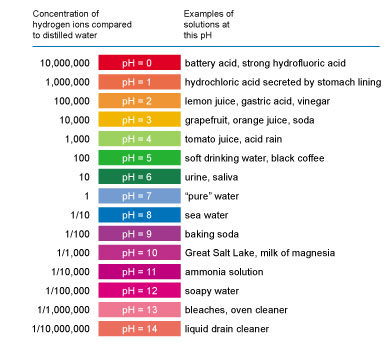
\includegraphics[width=\textwidth]{./Planning/Images/pHScale.jpg}
    \caption{The pH scale} \label{fig:pH Scale}
\end{figure}

The pH scale is a man made scale which is used to measure the concentration of hydrogen ions, each concentration is given a corresponding place on the scale (pH). pH is mathematically defined as the negative logarithm of the hydrogen ion concentration. As a result of this we can determine that the pH scale is logarithmic, therefore each value above/below the neutral value (7) is ten times more basic/acidic respectively. For example pH 6 is ten times as acidic as pH 7  and pH 5 is one hundred times as acidic than pH 7. The mathematical equation for working out pH is illistrated below.

\begin{itemize}
\item $pH = - log [H^+]$
\end{itemize}

There are many indicators used to find out the pH of substances. A table of common indicators with their properties are displayed in the table below.

\begin{figure}[H]
    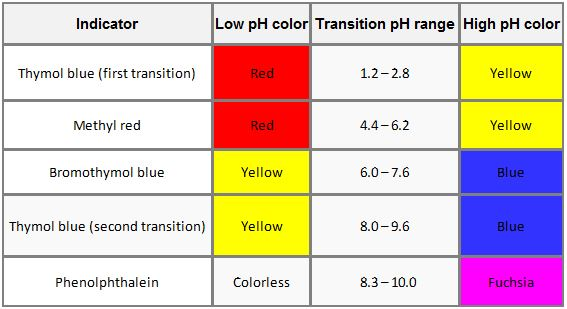
\includegraphics[width=\textwidth]{./Planning/Images/Indicators.jpg}
    \caption{List of pH Indicators} \label{fig:pH Indicators}
\end{figure}

Universal indicator contains all of the chemicals above, all mixed into a single solution or into universal indicator paper. This allows for a continuous color change from about pH 2 to pH 10. Visual comparison of the colour of the universal indicator and a standard colour chart give a rough reading of the pH of the substance being measured, usually to the nearest whole number. 


	\subsection{Acids}

The Brønsted–Lowry theory defines an acid as a proton $(H^+)$ donor. 

-Weak/strong (organic/inorganic) (dissociation)
-Low conc/High conc



	\subsection{Catalysts}








	\subsection{Enthalpy Level Diagrams}	







	\subsection{Transition Metal Catalysts}



	\subsection{D-Orbitals}



	\subsection{Complexes and their Properties}


\section{Inventory}

	\subsection{Equipment List}
\begin{itemize}
\item 250 $cm^3$ conical flask.
\item Bung fitted to a glass tube.
\item Burette.
\end{itemize}

	\subsection{Chemical List}
\begin{itemize}
\item Distilled Water.
\item 0.20 mol dm$^-3$ Copper Sulfate ${_(aq)}$.
\item 1.0 mol dm$^-3$ Sulfuric Acid${_(aq)}$.
\item Granulated Zinc${_(s)}$.
\item Mixture of Different Catalysts.
\end{itemize}



\section{Methods}

	\subsection{Chosen Method}

\textbf{Setting Up}

\begin{enumerate}
\item Fill the Burette with distilled water.
\item Fit the bung (fitted with glass tube) into the conical flask.
\item Fit the inverted Burette to the end of the glass tube.
\end{enumerate}

\textbf{Carrying out the Experiment}

\begin{enumerate}
\item Remove the bung from the conical flask and pour 30 cm$^3$ of distilled water and 10 cm$^3$ of sulfuric acid into the conical flask.
\item Weigh out 1.0 g of granulated zinc.
\item Add the measured 1.0 g of granulated zinc to the conical flask.
\item Place the bung back in the conical flask.
\item Record the volume of hydrogen produced in cm$^3$ every 30 seconds for 5 minutes from the burette markings to 1 decimal place.
\item Repeat the experiment but use 30 cm$^3$ of copper sulfate instead of distilled water.
\end{enumerate} 

\textbf{Interpreting the Data (as discussed before)}

\begin{enumerate}
\item Plot a graph of the volume of hydrogen against time.
\item From the graph draw a tangent to the line at the initial point.
\item Calculate the gradient of the tangent by using the equation: 
\item The gradient is equal to the rate of reaction.
\end{enumerate}



	\subsection{Justification of Chosen Method}

In addition to the method discussed above, there are two other methods which would allow me to carry out my experiment:
\begin{itemize}
\item The Gas Syringe Method
\item The Mass Change Method 
\end{itemize}

Below, the methods are explained:

\textbf{Gas Syringe Method}



Setting up involves a similar set up to my chosen method, but the gas syringe replaces the burette. This is shown below:
\begin{figure}[H]
    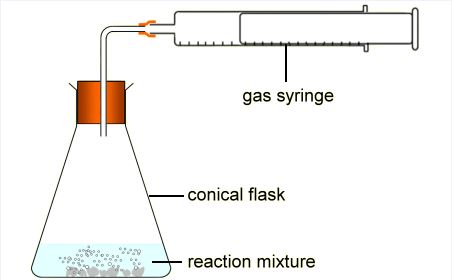
\includegraphics[width=\textwidth]{./Planning/Images/GasSyringe.jpg}
    \caption{Gas Syringe Equipment} \label{fig:Gas Syringe}
\end{figure}

Carrying out the method is precisely the same as my chosen method except a reading is taken from the gas syringe instead of the burette. This is precisely the reason I have chosen to not use this method. The gas syringes available to me have graduations every 1 ml, whereas the burrettes available to me have graduations every 0.1 ml. Therefore the accuracy of my readings will be greater using the burette method and consequently I have chosen the burette method ovet the gas syring method. 

\textbf{Mass Change Method}

Setting up this method involves:
\begin{itemize}
\item Balance (reading to 0.01 g)
\item Conical Flask
\item Cotton Wool
\end{itemize}

\begin{figure}[H]
    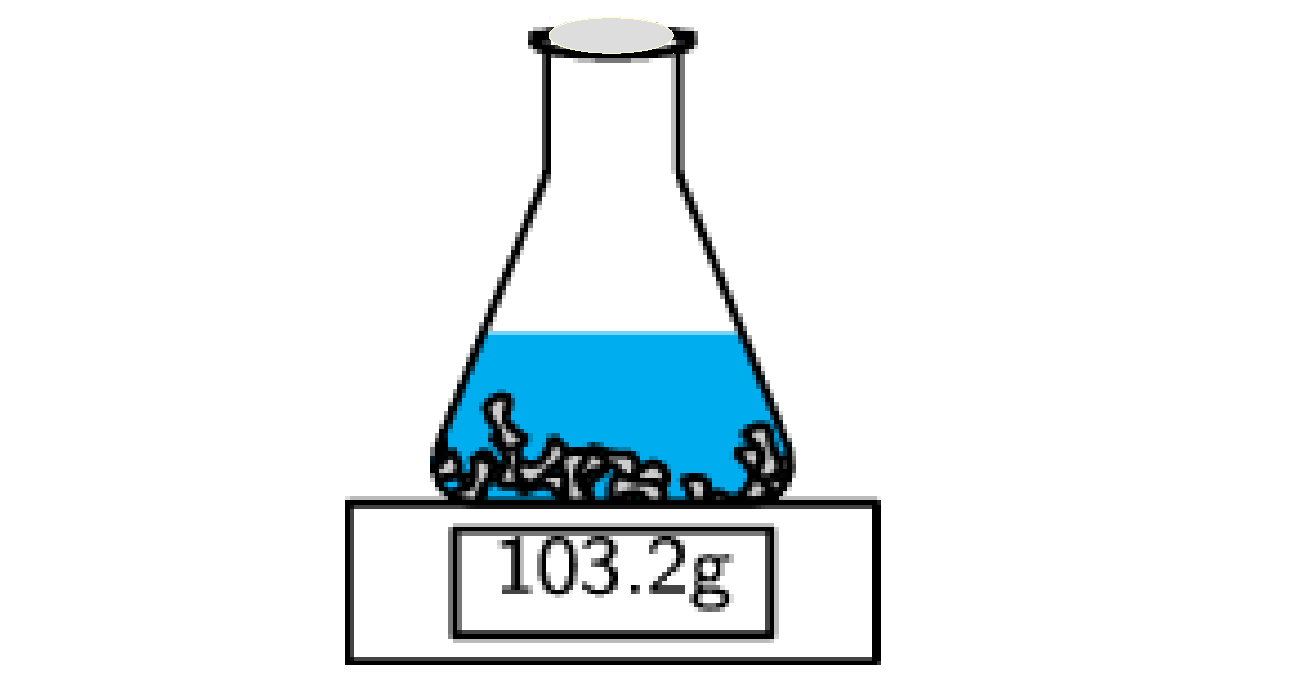
\includegraphics[width=\textwidth]{./Planning/Images/MassChange.pdf}
    \caption{Mass Change Equipment} \label{fig:Mass Change}
\end{figure}


Carrying out this method involves:

\begin{enumerate}
\item Zero the Balance.
\item Pour 30 cm$^3$ of distilled water and 10 cm$^3$ of sulfuric acid into the conical flask.
\item Take note of the Balance value + 1.0 g
\item Weigh out 1.0 g of granulated zinc.
\item Add the measured 1.0 g of granulated zinc to the conical flask.
\item Place the cotton wool in the conical flask to stop acid 'spray' excaping.
\item Record the loss in mass in grams every 30 seconds for 5 minutes to 2 decimal places.
\item Repeat the experiment but use 30 cm$^3$ of copper sulfate instead of distilled water.
\end{enumerate} 

I have chosen not to carry out this method as the balance will be a lot more sensitive to the environment and there will be room for a lot more human error. For example, left over residue could land on the scales and scew the results during the experiment. 


\begin{landscape}

\section{Risk Assessment}

\begin{center}
\begin{longtable}{|p{1.5cm}|p{1.5cm}|p{3cm}|p{3cm}|p{3cm}|p{3cm}|p{2cm}|}
    \hline
 \textbf{Name of Chemical} & \textbf{Source of Information} & \textbf{Hazards} & \textbf{Risks} & \textbf{Control Measures} & \textbf{Disposal Method} & \textbf{Emergency Procedures} \\ \hline

Copper Sulfate (aq) &
CLEAPSS Hazcards &
\begin{itemize}
\item Harmful
\item Dangerous for the Environment \end{itemize} &
\begin{itemize}
\item Harmful if swallowed
\item Irritating to eyes and skin \end{itemize} &
\begin{itemize}
\item Do not put near mouth
\item Use gloves
\item Use goggles
\item Keep away from water, unless intended. \end{itemize} & 
Dissolve 64 g in 1 litre of water before pouring the solution down a foulwater drain. This disposal procedure should be kept to a minimum. &
Seek medical attention. Wash contaminated area. \\ \hline

Hydrated Copper Sulfate (s) &
CLEAPSS Hazcards &
\begin{itemize}
\item Harmful
\item Dangerous for the Environment \end{itemize} &
\begin{itemize}
\item Harmful if swallowed
\item Irritating to eyes and skin \end{itemize} &
\begin{itemize}
\item Do not put near mouth
\item Use gloves
\item Use goggles
\item Label: Harmful, if above 1 moldm$^-3$ \end{itemize} &
Crystals may be used for solutions. Dilute to less than 0.4 mol dm$^-3$ or dissolve 100 g in 1 litre of water before pouring the solution down a foul-water drain. This disposal procedure should be kept to a minimum . &
Seek medical attention. Wash contaminated area. \\ \hline



Sulfuric Acid (aq) &
CLEAPSS Hazcards &
\begin{itemize}
\item Corrosive
\item Irritant \end{itemize} &
Causes serious burns & 
\begin{itemize}
\item Label: Irritant, if above 0.5 moldm$^-3$
\item Label: Corrosive, if above 1.5 moldm$^-3$
\item Wear gloves
\item Wear goggles \end{itemize} &
Add slowly no more than 10 cm$^3$ of concentrated sulfuric(VI) acid to 1 litre of 1 mol dm$^-3$ sodium carbonate solution (containing indicator) which should be constantly stirred. Let the mixture cool (or add ice), before adding more acid. Pour the solution down a foul-water drain. & 
Remove contaminated clothing and quickly wipe as much liquid as possible off the skin with a dry cloth before drenching the area with a large excess of water. If a large area is affected or blistering occurs, seek medical attention. \\ \hline

Granulated Zinc (s) &
CLEAPSS Hazcards &
\begin{itemize}
\item Low Hazard \end{itemize} &
N/A &
Place in normal refuse &
N/A &
N/A \\ \hline

\end{longtable}
\label{tab:Risk Assessment Table}

\end{center}


\end{landscape}



